\subsection{Verification of our implemented of the Cross-entropy method \label{varifyofce}}

Because the \shark\ library already contains an implementation of 
CMA-ES, but not an implementation of the Cross-entropy method, we extended the library
with our own implementation of the algorithm.\\
In order to verify the correctness of the implementation, 
we used the same experiments as used by 
Christophe Thiery and Bruno Scherrer \citep{thiery:09}. 
These experiments were used by Thiery and Scherrer to 
verify their own Cross-entropy method implementation with various types of noise correction. 
Therefore, we will perform the same experiments to verify our 
own contribution to the \shark\  library, by trying to achieve the same results.\\
\\
The setup is mirrored from the paper \citep{thiery:09}, 
with 100 agents ($\populationSize = 100$) per iteration,
and using the $\offspringNumber = 10$ best vectors
for the update step. After each iteration, 
an agent with the updated mean 
plays 30 games and the mean of these scores are recorded for the
learning curve.\\
During evaluation each agent plays one game, that is $\numberOfEvaluations = 1$.
A minor derivation from the figures present in \citep{thiery:09}, is 
the unit along the x-axis in the learning curve plots indicates 
the iteration number. As the experiments in this two algorithms
width variable population sizes are compared, the x-axis in all plots
indicated the number of Tetris games played during the learning. In one 
generation $\populationSize$ agents each play $\numberOfEvaluations$ games and hence
advance the x-axis by $\populationSize \numberOfEvaluations$.\\

\begin{figure}[H]
\begin{center}
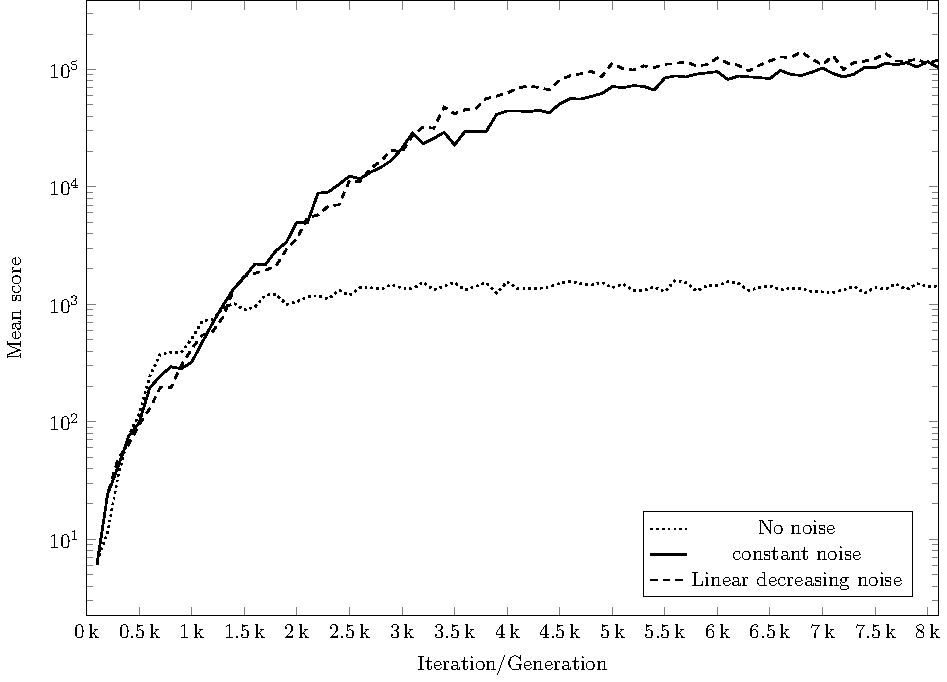
\includegraphics[scale=0.8]{plots/meansPlot}
\end{center}
\caption{Cross-Entropy mean performance \label{fig:cemean}}
\end{figure}

\clearpage
\begin{figure}[H]
\begin{center}
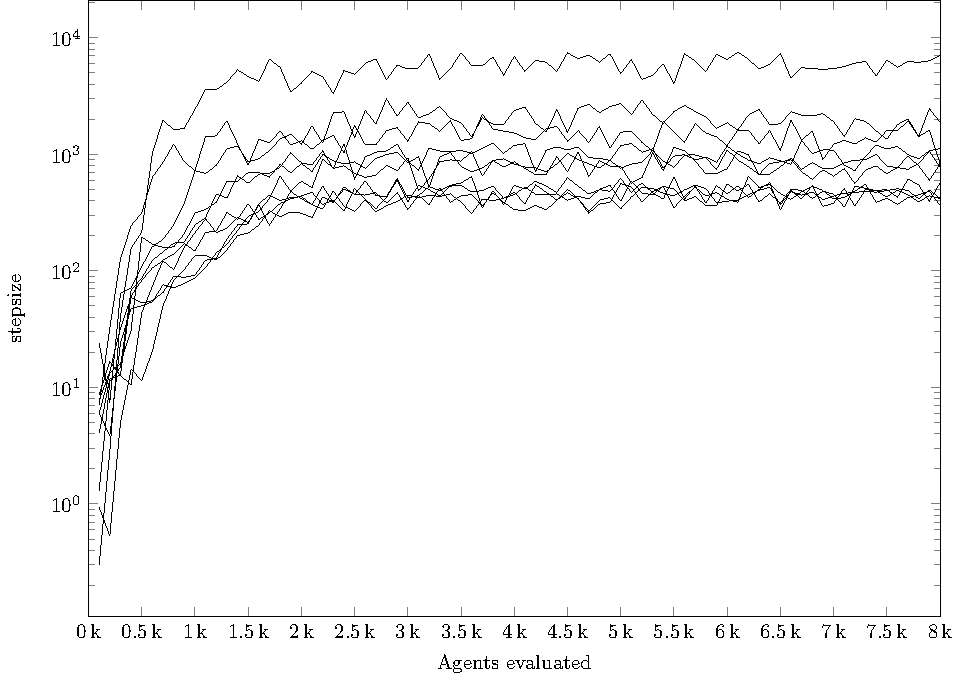
\includegraphics[scale=0.48]{plots/noNoisePlot}
\end{center}
\caption{No noise \label{fig:ceNoNoise}}
\end{figure}
\begin{figure}[H]
\begin{center}
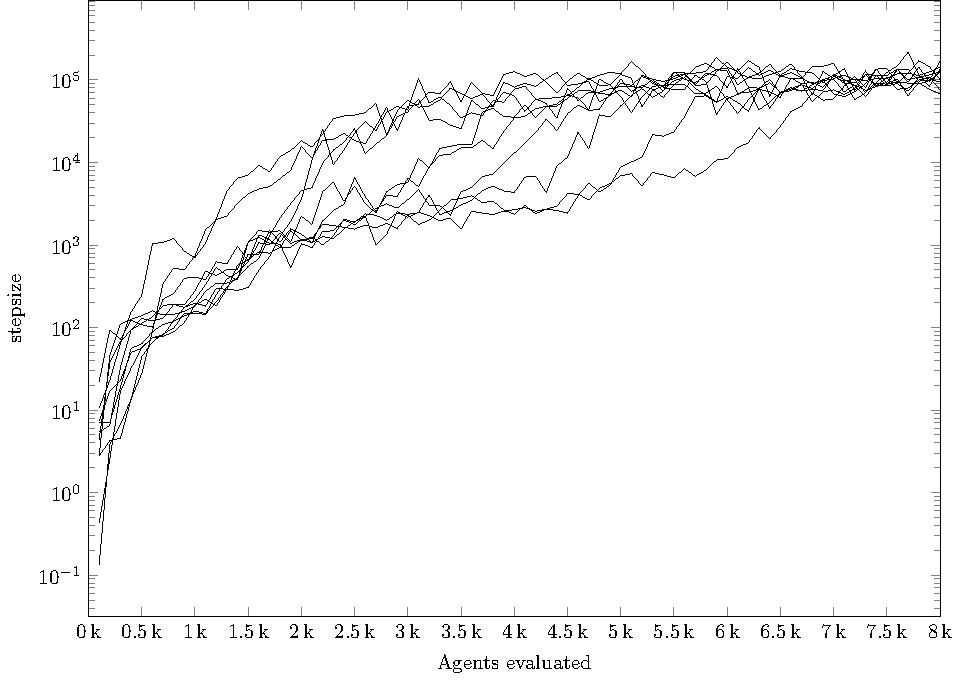
\includegraphics[scale=0.48]{plots/constantNoisePlot}
\end{center}
\caption{Constant noise \label{fig:ceCnstantNoise}}
\end{figure}
\begin{figure}[H]
\begin{center}
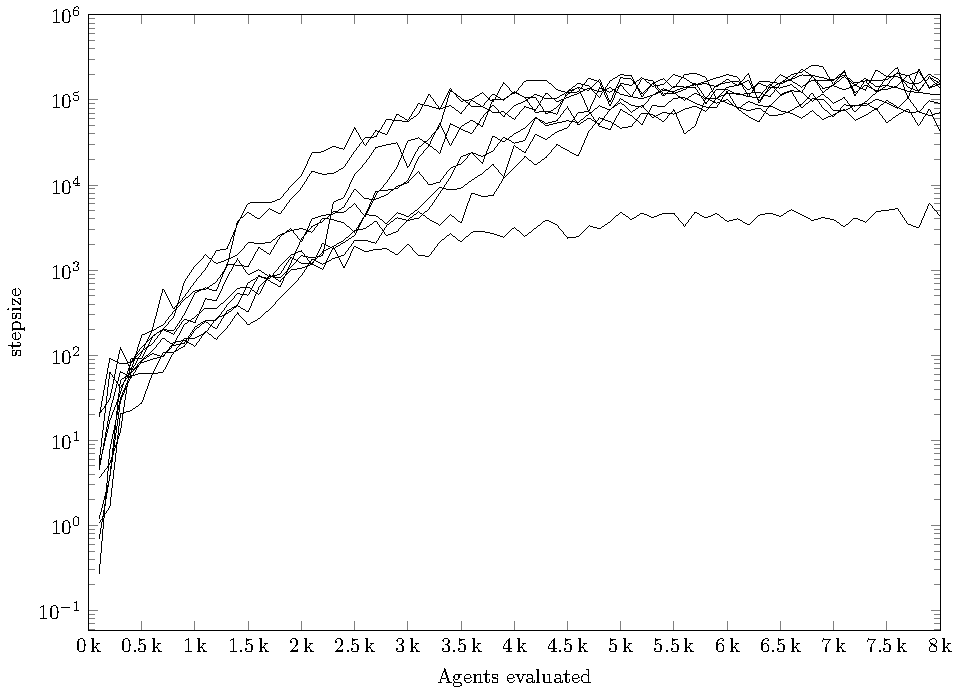
\includegraphics[scale=0.48]{plots/linearNoisePlot}
\end{center}
\caption{Linear decreasing noise \label{fig:ceLinNoise}}
\end{figure}

Figure \ref{fig:ceNoNoise}, \ref{fig:ceCnstantNoise} and
\ref{fig:ceLinNoise} shows 10 runs of each noise type. Figure
\ref{fig:cemean} shows the mean graph for each of the noise types.
The goal of these experiments were to replicate the experiments 
reported in \citep{thiery:09}. As the results seen from our experiments
to a high degree resemble those reported by Thiery et. al, we conclude
that our Cross-entropy method implementation works similar to theirs.\\
\\
When evaluating the score of the agent we also want to compute the confidence
interval in verifying the implementation of the Cross-entropy method. The mean agent plays 30 games
which leads to a confidence interval of $\pm36\%$ around the estimated mean,
which is similar to the confidence intervals in \citep{scherrer2009}.\\
By looking at the individual graphs for the different noise types 
(Figure \ref{fig:ceNoNoise}, \ref{fig:ceCnstantNoise} and
\ref{fig:ceLinNoise}), we get the following average scores.\\
\\
\textbf{Without noise (figure \ref{fig:ceNoNoise})}: The learning curve
stabilizes after 1,500 agents evaluated. And as it can be observed the
score variates much for the different executions between a score of 300 and 6,000
rows. This results in an average score of 1,400$\pm36\%$ rows.\\
\textbf{Constant noise (figure \ref{fig:ceCnstantNoise})}: 
The 10 executions reaches equivalent performances at some point, 
with a score between
54,000 and 154,000. This results in an average score of 105,000$\pm36\%$ rows.\\
\textbf{Linear decreasing noise (figure \ref{fig:ceLinNoise})}:
Most of the executions of this noise type settles around 200,000.
However, a single execution settled at a score of only around 5,000.
The mean performance of this noise type yielded a score of
120,000$\pm36\%$ \\

Based on the mean graphs and confidence interval compared to other papers, we can
hereby verify that our implementation of the Cross-entropy method works as intended. Even though the
experiments with linear decreasing noise in this case seems to outperform
the constant noise, other runs with linear decreasing noise ended in a mean 
performance of only 90,000$\pm36\%$. Yet, the constant noise is both from our
own experiments, and described in other research, noted to be the most reliable
noise type for reaching high scoring controllers \citep{scherrer2009}. 
Due to this, the constant noise is used in the 
benchmarking against CMA-ES.\\



